
\documentclass{beamer}
\usepackage[latin1]{inputenc}
%\usetheme{Montpellier}
%\usetheme{Boadilla}
%\usecolortheme[RGB={204,51,255}]{structure}
%\usecolortheme[named=purple]{structure}
\usecolortheme[RGB={62,128,62}]{structure}
%\definecolor{dark}{rgb}{0.3,0.15,0.3}
%\definecolor{light}{rgb}{0.8,0.6,0.8}
%\definecolor{reddish}{rgb}{.5,0.15,0.15}
\definecolor{dark}{rgb}{0.5,0.3,0.4}
%\definecolor{light}{rgb}{0.8,0.6,0.8}
\definecolor{reddish}{rgb}{.7,0.25,0.25}
\definecolor{greenish}{rgb}{.25,0.7,0.25}
\definecolor{blueish}{rgb}{.25,0.25,0.7}
\definecolor{purple}{rgb}{.5,0.0,0.5}
\usepackage{graphicx}
\usepackage{pstricks}

\usepackage{amsmath}
\setbeamertemplate{navigation symbols}{}

\newcommand{\crish}{\color{reddish}}
\newcommand{\cbla}{\color{black}}
\newcommand{\cred}{\color{red}}
\newcommand{\cblu}{\color{blue}}

\newcommand{\sm}{\color{reddish}$}
\newcommand{\fm}{$\color{black}}


\usepackage{tikz}
\usetikzlibrary{arrows,decorations.markings,positioning}
\usepackage{epstopdf}

\title[Motivating Shannon's Entropy: lecture 1]{Information Theory lecture 1}
\author{COMSM0075 Information Processing and Brain}
\institute{\texttt{comsm0075.github.io}}
\date{September 2020}

\begin{document}

\maketitle


\begin{frame}{Information Theory}
\begin{quote}  
The theory of information is a theory of communication.
\end{quote}
\end{frame}


\begin{frame}{a theory of communication}
  \begin{center}
  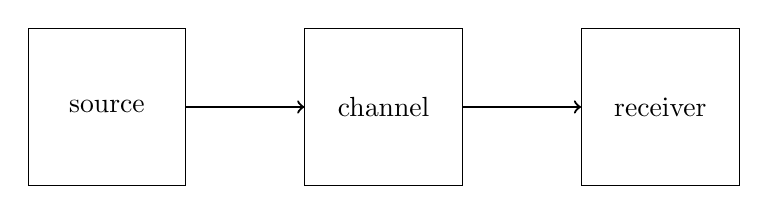
\begin{tikzpicture}
    \node[rectangle,draw,minimum size=2cm](source){source};
    \node[rectangle, minimum size=2cm,right = 1.5cm of source, draw](channel){channel};
    \node[rectangle, right = 1.5cm of channel,draw,minimum size=2cm](receiver){receiver};
    \draw(source) edge[->,thick] (channel);
    \draw(channel) edge[->,thick] (receiver);
  \end{tikzpicture}
  \end{center}
\end{frame}

\begin{frame}{randomness}
\begin{center}  
    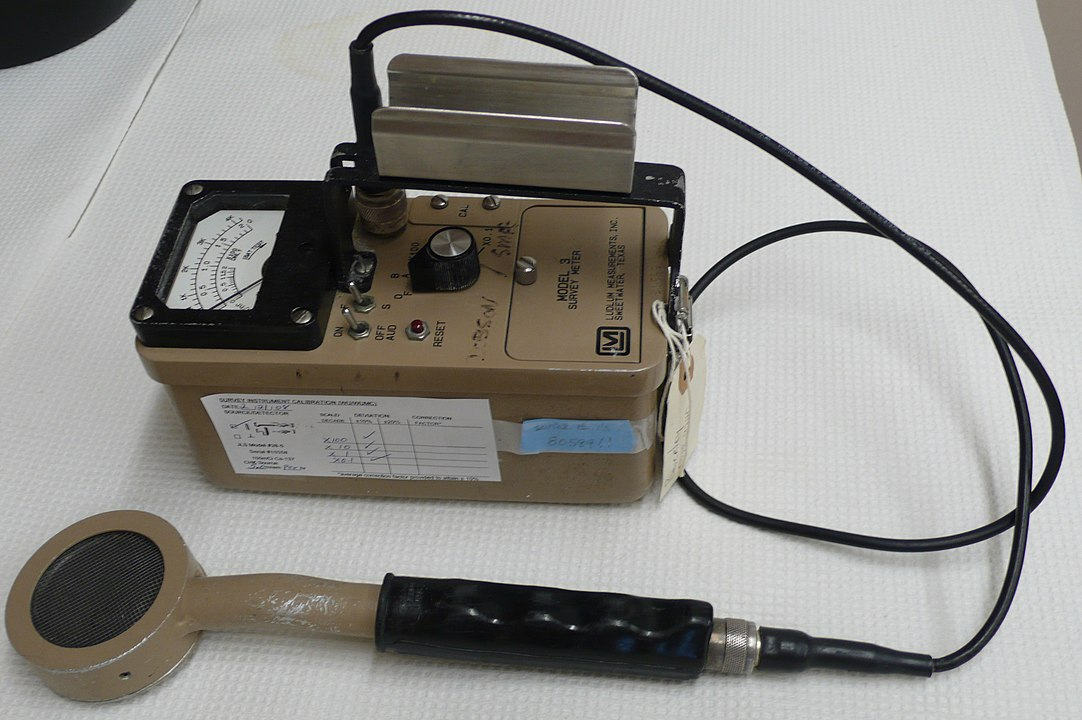
\includegraphics[width=10cm]{geiger_counter.jpg}
\end{center}
  \vfill
\tiny{Image from wikipedia.}
\end{frame}

\begin{frame}{unexpectedness}
\begin{center}  
\Huge{2020}
\end{center}
\end{frame}

\begin{frame}{a theory of communication}
  \begin{center}
  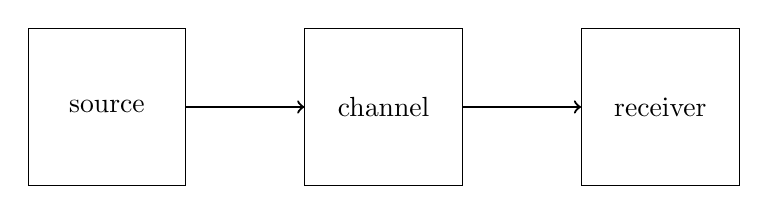
\begin{tikzpicture}
    \node[rectangle,draw,minimum size=2cm](source){source};
    \node[rectangle, minimum size=2cm,right = 1.5cm of source, draw](channel){channel};
    \node[rectangle, right = 1.5cm of channel,draw,minimum size=2cm](receiver){receiver};
    \draw(source) edge[->,thick] (channel);
    \draw(channel) edge[->,thick] (receiver);
  \end{tikzpicture}
  \end{center}
\end{frame}

\begin{frame}{film  recommendations}
  \begin{center}
    
\includegraphics[width=10cm]{stars.png}
  \end{center}
\end{frame}

\begin{frame}{film  recommendations are bad}
 \begin{center}
    
\includegraphics[width=10cm]{netflix_recommends.png}
 \end{center}
 \end{frame}

\begin{frame}{a theory of communication}
  \begin{center}
  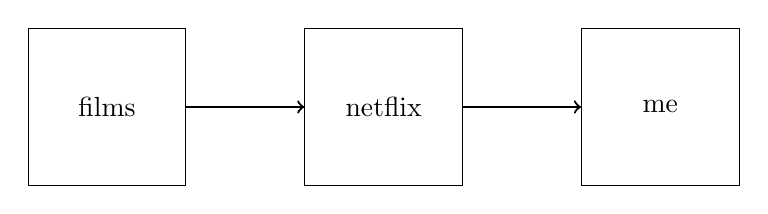
\begin{tikzpicture}
    \node[rectangle,draw,minimum size=2cm](source){films};
    \node[rectangle, minimum size=2cm,right = 1.5cm of source, draw](channel){netflix};
    \node[rectangle, right = 1.5cm of channel,draw,minimum size=2cm](receiver){me};
    \draw(source) edge[->,thick] (channel);
    \draw(channel) edge[->,thick] (receiver);
  \end{tikzpicture}
  \end{center}
\end{frame}

\begin{frame}{a theory of communication}
  \begin{center}
  \begin{tikzpicture}
    \node[rectangle,draw,minimum size=2cm](source){films};
    \node[rectangle, minimum size=2cm,right = 1.5cm of source, draw](channel){
    
\includegraphics[width=1.75cm]{netflix_recommends.png}
    };
    \node[rectangle, right = 1.5cm of channel,draw,minimum size=2cm](receiver){me};
    \draw(source) edge[->,thick] (channel);
    \draw(channel) edge[->,thick] (receiver);
  \end{tikzpicture}
  \end{center}
\end{frame}

\begin{frame}{film  recommendations are bad}
 \begin{center}
    
\includegraphics[width=10cm]{netflix_recommends.png}
 \end{center}
 \end{frame}

\begin{frame}{Netflix Prize}
  \begin{center}
    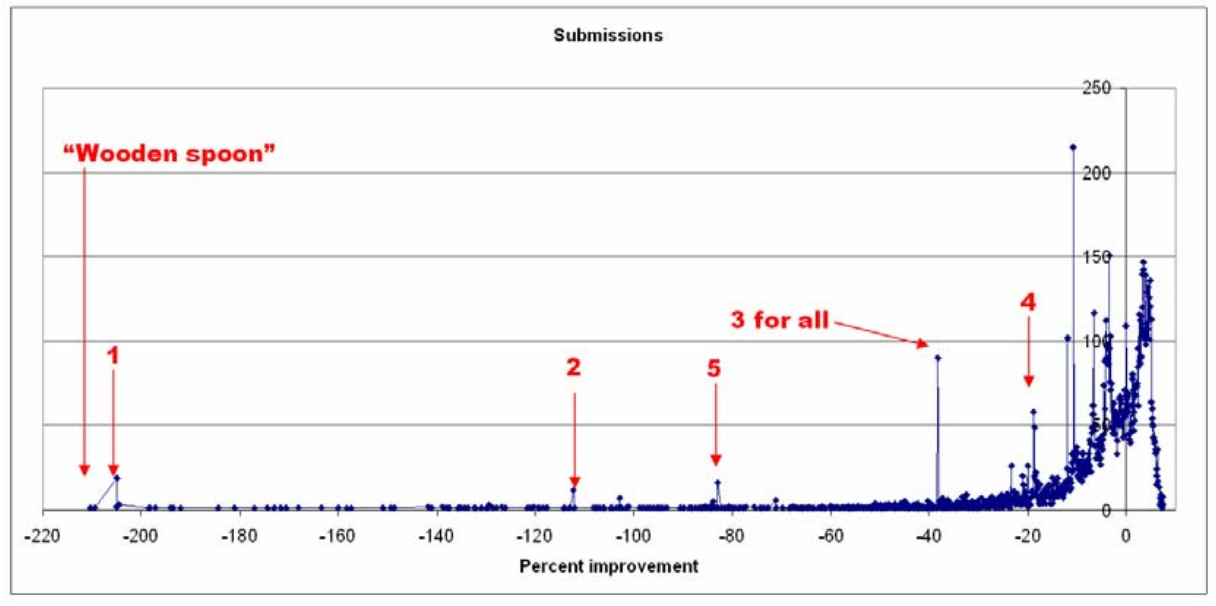
\includegraphics[width=10cm]{netflix_prize.png}
  \end{center}
  \vfill
\tiny{Bennett, James, and Stan Lanning. "The netflix prize." Proceedings of KDD cup and workshop. Vol. 2007. 2007.}
\end{frame}


\begin{frame}{Netflix Prize}
  \begin{center}
    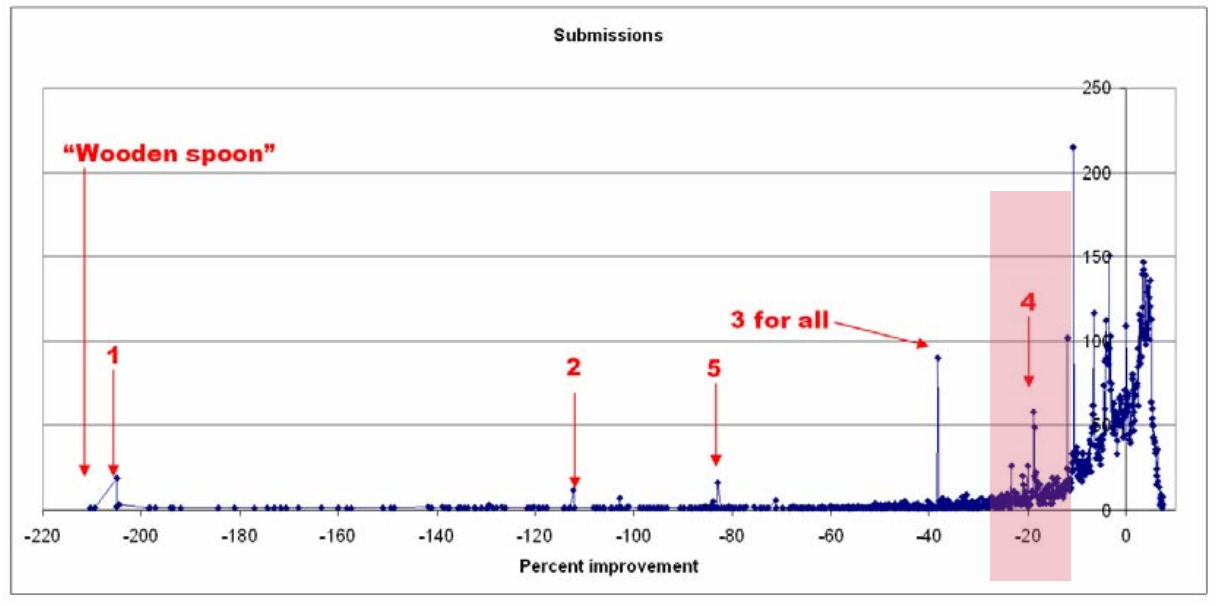
\includegraphics[width=10cm]{netflix_prize_1.png}
  \end{center}
  \vfill
\tiny{Bennett, James, and Stan Lanning. "The netflix prize." Proceedings of KDD cup and workshop. Vol. 2007. 2007.}
\end{frame}

\begin{frame}{film  recommendations}
  \begin{center}
    
\includegraphics[width=10cm]{stars.png}
  \end{center}
\end{frame}

%\begin{frame}{Netflix Prize}
%  \begin{center}
%    
\includegraphics[width=10cm]{napoleon.jpg}
%  \end{center}
%\end{frame}

\begin{frame}{average star ratings}
  \begin{center}
    \begin{tabular}{l|l}
      \hline
      1 star&0.016\\
      2 star&0.310\\
      3 star&0.627\\
      4 star&0.057\\
      \hline
    \end{tabular}
  \end{center}
\end{frame}

\begin{frame}{the average star ratings mean something}
  \begin{center}
    
\includegraphics[height=5cm]{avia_vampire_hunter.jpg}
    
\includegraphics[height=5cm]{hedwig.jpg}
  \end{center}
\end{frame}


\begin{frame}{mostly though they tell you it's an `ok' film}
  \begin{center}
    \begin{tabular}{l|l}
      \hline
      1 star&0.016\\
      2 star&0.310\\
      \textbf{3 star}&\textbf{0.627}\\
      4 star&0.057\\
      \hline
    \end{tabular}
  \end{center}
\end{frame}

\begin{frame}{a theory of communication}
  \begin{center}
  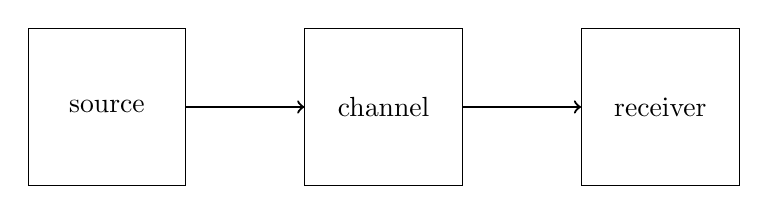
\begin{tikzpicture}
    \node[rectangle,draw,minimum size=2cm](source){source};
    \node[rectangle, minimum size=2cm,right = 1.5cm of source, draw](channel){channel};
    \node[rectangle, right = 1.5cm of channel,draw,minimum size=2cm](receiver){receiver};
    \draw(source) edge[->,thick] (channel);
    \draw(channel) edge[->,thick] (receiver);
  \end{tikzpicture}
  \end{center}
\end{frame}


\begin{frame}{a theory of communication}
  \begin{center}
  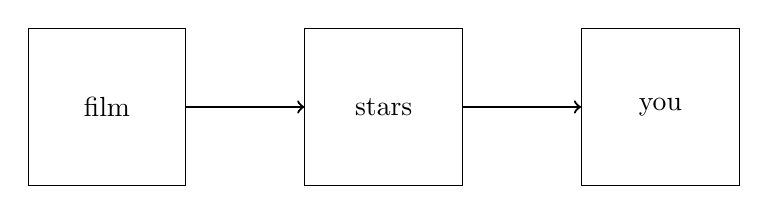
\begin{tikzpicture}
    \node[rectangle,draw,minimum size=2cm](source){film };
    \node[rectangle, minimum size=2cm,right = 1.5cm of source, draw](channel){stars};
    \node[rectangle, right = 1.5cm of channel,draw,minimum size=2cm](receiver){you};
    \draw(source) edge[->,thick] (channel);
    \draw(channel) edge[->,thick] (receiver);
  \end{tikzpicture}
  \end{center}
\end{frame}


\begin{frame}{a theory of communication}
  \begin{center}
  \begin{tikzpicture}
    \node[rectangle,draw,minimum size=2cm](source){film };
    \node[rectangle, minimum size=2cm,right = 1.5cm of source, draw, inner sep = 0pt](channel){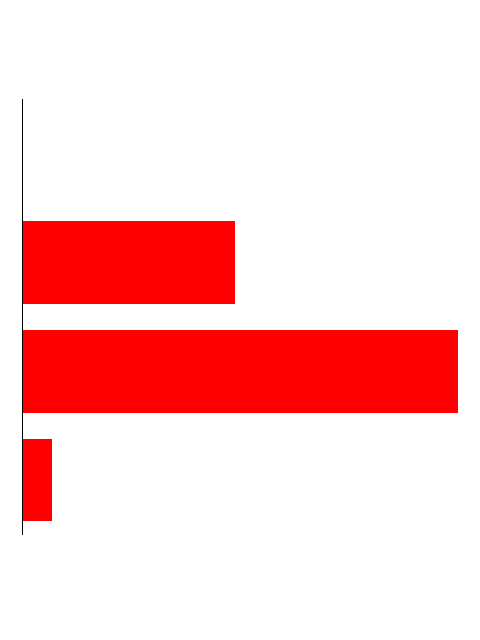
\includegraphics[width=1.45cm]{ratings_rotated.png}};
    \node[rectangle, right = 1.5cm of channel,draw,minimum size=2cm](receiver){you};
    \draw(source) edge[->,thick] (channel);
    \draw(channel) edge[->,thick] (receiver);
  \end{tikzpicture}
  \end{center}
\end{frame}

\begin{frame}{the fable of Stefan}
  \begin{center}
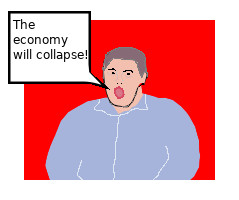
\includegraphics[width=5cm]{boring_man.jpg}
\end{center}
  \end{frame}


\begin{frame}{a theory of communication}
  \begin{center}
  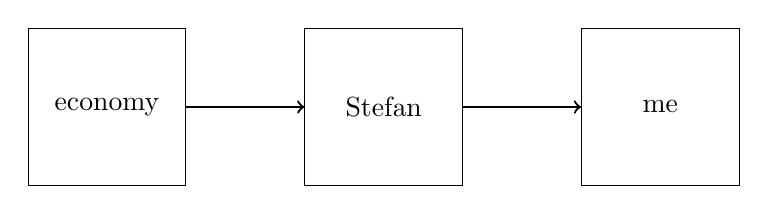
\begin{tikzpicture}
    \node[rectangle,draw,minimum size=2cm](source){economy };
    \node[rectangle, minimum size=2cm,right = 1.5cm of source, draw](channel){Stefan};
    \node[rectangle, right = 1.5cm of channel,draw,minimum size=2cm](receiver){me};
    \draw(source) edge[->,thick] (channel);
    \draw(channel) edge[->,thick] (receiver);
  \end{tikzpicture}
  \end{center}
\end{frame}

\begin{frame}{a theory of communication}
  \begin{quote}
    The theory of information starts with an attempt to allow us to
quantify the informativeness of information, but not its salience or
validity.
  \end{quote}
  \end{frame}

\begin{frame}{Shannon's entropy}
  For a finite discrete distribution with random variable \sm X\fm,
  possible outcomes \sm\{x_1,x_2,\ldots x_n\}\in\mathcal{X}\fm{} and a
  probability mass function \sm p_X\fm{} giving probabilities \sm p_X(x_i)\fm, the
  entropy is
\crish
  $$
H(X)=-\sum_{x_i\in \mathcal{X}}{p_X(x_i)\log_2p_X(x_i)}
  $$
\cbla
\end{frame}

\begin{frame}{Shannon's entropy}
  For a finite discrete distribution with random variable \sm X\fm,
  possible outcomes \cblu $\{x_1,x_2,\ldots x_n\}\in\mathcal{X}$\cbla{} and a
  probability mass function \sm p_X\fm{} giving probabilities \sm p_X(x_i)\fm, the
  entropy is
\crish
  $$
H(X)=-\sum_{x_i\in \mathcal{X}}{p_X(x_i)\log_2p_X(x_i)}
  $$
\cbla
\end{frame}

\begin{frame}{Shannon's entropy}
  For a finite discrete distribution with random variable \sm X\fm,
  possible outcomes \sm\{x_1,x_2,\ldots x_n\}\in\mathcal{X}\fm{} and a
  probability mass function \sm p_X\fm{} giving probabilities \cblu$ p_X(x_i)$\cbla, the
  entropy is
\crish
  $$
H(X)=-\sum_{x_i\in \mathcal{X}}{p_X(x_i)\log_2p_X(x_i)}
  $$
\cbla
\end{frame}

\begin{frame}{example calculation - netflix}
  \begin{center}
    \begin{tabular}{l|l}
      \hline
      1 star&0.016\\
      2 star&0.310\\
      3 star&0.627\\
      4 star&0.057\\
      \hline
    \end{tabular}
  \end{center}
  \crish
  \begin{multline*}
    H(X)=-0.016\log_2{0.016}-0.31\log_2{0.31}\\
    -0.627\log_2{0.627}-0.057\log_2{0.057}\approx 1.28
\end{multline*}
\cbla
\end{frame}  


\begin{frame}{example calculation - netflix}
  Imagine instead all rankings are equally likely
    \begin{center}
    \begin{tabular}{l|l}
      \hline
      1 star&0.25\\
      2 star&0.25\\
      3 star&0.25\\
      4 star&0.25\\
      \hline
    \end{tabular}
  \end{center}
  \crish
  $$
H(X)=-4\times 0.25\log_2{0.25}=2
  $$
\cbla
\end{frame}  


\begin{frame}{example calculation - netflix}
  Imagine instead everything gets one stars, the Stefan-like case
    \begin{center}
    \begin{tabular}{l|l}
      \hline
      1 star&1\\
      2 star&0\\
      3 star&0\\
      4 star&0\\
      \hline
    \end{tabular}
  \end{center}
  \crish
  $$
H(X)=-\log_2{1}=0
  $$
\cbla
\end{frame}

\begin{frame}{example calculation - netflix}
  \begin{itemize}
  \item deterministic \crish $H(X)=0$\cbla
  \item actual \crish $H(X)\approx 1.28$\cbla
  \item completely random \crish $H(X)=2$\cbla
\end{itemize}
\end{frame}

\begin{frame}{0 or 1.28 or 2}
  \begin{center}
  \begin{tikzpicture}
    \node[rectangle,draw,minimum size=2cm](source){films};
    \node[rectangle, minimum size=2cm,right = 1.5cm of source, draw](channel){
    
\includegraphics[width=1.75cm]{stars.png}
    };
    \node[rectangle, right = 1.5cm of channel,draw,minimum size=2cm](receiver){you};
    \draw(source) edge[->,thick] (channel);
    \draw(channel) edge[->,thick] (receiver);
  \end{tikzpicture}
  \end{center}
\end{frame}


\end{document}

